\section{Document organization}
This thesis is organised into two parts:
%An overview of the chapters can be seen in Figure \ref{fig:chapter-overview}.

The first part (\ref{part1}) provides a literature review of state of the art techniques in robot programming ({\chapt{chap:Sota}}), followed by an overview of Automated Planning ({\chapt{chap:Sota-AP}}).

The second part (\ref{part2}) presents our contributions involving iRoPro, the proposed end-user robot programming framework ({\chapt{chap:Contribution}}). 
We first conduct qualitative experiments and present experimental findings on user acceptance and issues encountered when introduced to Automated Planning concepts ({\chapt{chap:Pre-Experiments}}).
We then focus on evaluating our goal-oriented end-user robot programming approach and present our work on shelf organising tasks to simultaneous program goals and actions by demonstration ({\chapt{chap:OrganisingTasks}}).
Our main contribution is an end-to-end system implementation of iRoPro. We present details on the implementation and the system and user evaluation in {\chapt{chap:Implementation}}.

Finally, we conclude this thesis in {\chapt{chap:Conclusion}} and discuss possibilities for future work and research.

%
\tikzstyle{format} = [draw, thin, fill=blue!20]
\tikzstyle{medium} = [ellipse, draw, thin, fill=green!20, minimum height=2.5em]

\begin{figure}
	\begin{tikzpicture}[node distance=3cm, auto,>=latex', thick]
	% We need to set at bounding box first. Otherwise the diagram
	% will change position for each frame.
	\path[use as bounding box] (-1,0) rectangle (10,-2);
	\path[->]<1-> node[format] (tex) {.tex file};
	\path[->]<2-> node[format, right of=tex] (dvi) {.dvi file}
	(tex) edge node {\TeX} (dvi);
	\path[->]<3-> node[format, right of=dvi] (ps) {.ps file}
	node[medium, below of=dvi] (screen) {screen}
	(dvi) edge node {dvips} (ps)
	edge node[swap] {xdvi} (screen);
	\path[->]<4-> node[format, right of=ps] (pdf) {.pdf file}
	node[medium, below of=ps] (print) {printer}
	(ps) edge node {ps2pdf} (pdf)
	edge node[swap] {gs} (screen)
	edge (print);
	\path[->]<5-> (pdf) edge (screen)
	edge (print);
	\path[->, draw]<6-> (tex) -- +(0,1) -| node[near start] {pdf\TeX} (pdf);
	\end{tikzpicture}
\end{figure}


\begin{figure}[h]
	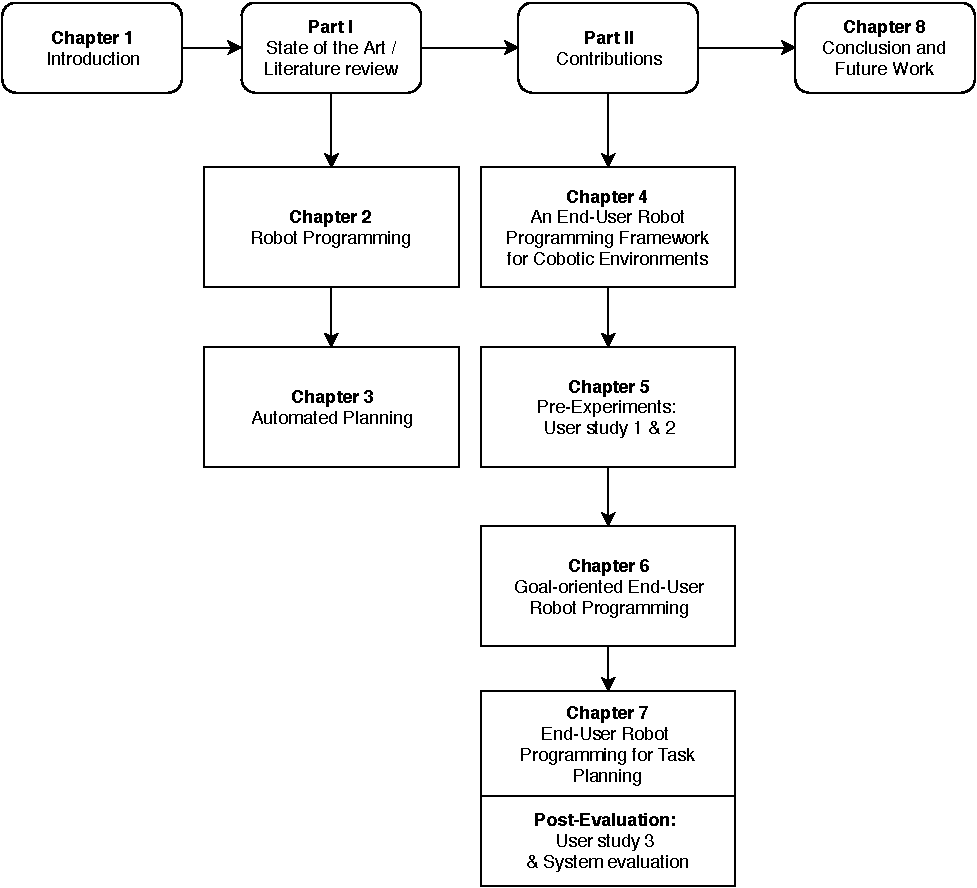
\includegraphics[width=\linewidth]{figures/chapter-overview.pdf}
	\caption{Overview of thesis chapters}
	\label{fig:chapter-overview}
\end{figure}
